\begin{figure}[!ht]
\centering
\figuretitle{Figure~\ref{fig:intra_dimer_interface_6OVW_vs_other_B_factor}}
\begin{fullpanelvar}
    \begin{emptypanel}{}
        %
        \node(pdb_6OVW)[inner sep=0pt,below right]{\includegraphics[height=1.125in,keepaspectratio]{../results/dimer_interface/output/deo_native_B_factor_cropped.png}};
        %
        \node(pdb_6OVW_caption)[below, inner sep=5pt] at (pdb_6OVW.south) {6OVW (1.88 \AA, This Study)};
        %
        \path (pdb_6OVW.east)++(-0.5,1) coordinate (pdb_6OVW_ROI_SE); 
        \node(pdb_6OVW_ROI) [fit={(pdb_6OVW.north) (pdb_6OVW_ROI_SE)}, dashedrectanglefit] {}; 
        %
        % Excluded: low-res
        %
        % \node(pdb_2vaf)[inner sep=0pt,right=0.75cm of pdb_6OVW]{\includegraphics[height=1.125in,keepaspectratio]{../results/dimer_interface/output/2vaf_B_factor_cropped.png}};
        % %
        % \node(pdb_2vaf_caption)[below, inner sep=5pt] at (pdb_2vaf.south) {2VAF (3.80 \AA)};
        %
        \node(pdb_3uom)[inner sep=0pt,right=0.75cm of pdb_6OVW]{\includegraphics[height=1.125in,keepaspectratio]{../results/dimer_interface/output/3uom_B_factor_cropped.png}};
        %
        \node(pdb_3uom_caption)[below, inner sep=5pt] at (pdb_3uom.south) {3UOM (2.015 \AA)};
        %
        \path (pdb_3uom.east)++(-0.75,1) coordinate (pdb_3uom_ROI_SE); 
        \path (pdb_3uom.north)++(-0.25,0) coordinate (pdb_3uom_ROI_NW); 
        \node(pdb_3uom_ROI) [fit={(pdb_3uom_ROI_NW) (pdb_3uom_ROI_SE)}, dashedrectanglefit] {}; 
        %
        \node(pdb_5crg)[inner sep=0pt,right=0.75cm of pdb_3uom]{\includegraphics[height=1.125in,keepaspectratio]{../results/dimer_interface/output/5crg_B_factor_cropped.png}};
        %
        \node(pdb_5crg_caption)[below, inner sep=5pt] at (pdb_5crg.south) {5CRG (1.970 \AA)};
        %
        \path (pdb_5crg.east)++(-0.5,1) coordinate (pdb_5crg_ROI_SE); 
        \node(pdb_5crg_ROI) [fit={(pdb_5crg.north) (pdb_5crg_ROI_SE)}, dashedrectanglefit] {}; 
        %
        %
        %
        \node(pdb_5crh)[inner sep=0pt,below=1cm of pdb_6OVW]{\includegraphics[height=1.125in,keepaspectratio]{../results/dimer_interface/output/5crh_B_factor_cropped.png}};
        %
        \node(pdb_5crh_caption)[below, inner sep=5pt] at (pdb_5crh.south) {5CRH (2.03 \AA)};
        %
        \path (pdb_5crh.east)++(-0.5,1) coordinate (pdb_5crh_ROI_SE); 
        \node(pdb_5crh_ROI) [fit={(pdb_5crh.north) (pdb_5crh_ROI_SE)}, dashedrectanglefit] {}; 
        %
        \node(pdb_5kn1)[inner sep=0pt,right=1cm of pdb_5crh]{\includegraphics[height=1.125in,keepaspectratio]{../results/dimer_interface/output/5kn1_B_factor_cropped.png}};
        %
        \node(pdb_5kn1_caption)[below, inner sep=5pt] at (pdb_5kn1.south) {5KN1 (2.137 \AA)};
        %
        \path (pdb_5kn1.east)++(-0.5,1) coordinate (pdb_5kn1_ROI_SE); 
        \node(pdb_5kn1_ROI) [fit={(pdb_5kn1.north) (pdb_5kn1_ROI_SE)}, dashedrectanglefit] {}; 
        %
        \node(pdb_5kn2)[inner sep=0pt,right=0.75cm of pdb_5kn1]{\includegraphics[height=1.125in,keepaspectratio]{../results/dimer_interface/output/5kn2_B_factor_cropped.png}};
        %
        \node(pdb_5kn2_caption)[below, inner sep=5pt] at (pdb_5kn2.south) {5KN2 (2.601 \AA)};
        %
        \path (pdb_5kn2.east)++(-0.5,1) coordinate (pdb_5kn2_ROI_SE); 
        \node(pdb_5kn2_ROI) [fit={(pdb_5kn2.north) (pdb_5kn2_ROI_SE)}, dashedrectanglefit] {}; 
        %                
        %
        %
        \draw [decorate,decoration={brace,amplitude=10pt,mirror,raise=4pt},yshift=0pt] ([shift={(1cm,0cm)}]pdb_5kn2.south east) -- ([shift={(1cm,4cm)}]pdb_5kn2.north east) node(group_label_tight) [black,midway,xshift=2.5cm,text width=3.5cm] {B-factor spectrum of chain A from tightly-packed dimers in published calsequestrin structures};
        %
        %
        %
        \draw[] ([yshift=-1cm]pdb_5crh.south west) -- ([yshift=-1cm]pdb_5kn2.south east);
        % [shift={(0.5,0.5)}]
        \node(spectrum_bar_tight)[inner sep=0pt] at ([yshift=-0.5cm]group_label_tight.south){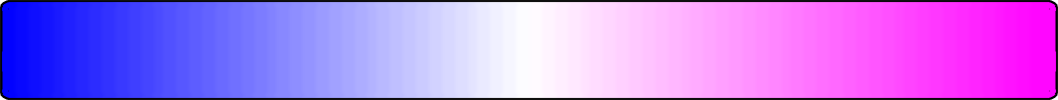
\includegraphics[width=\linewidth,height=0.1in,keepaspectratio]{../bin/colormaps/resource/pymol_blue_white_magenta_spectrum.png}};
        %
        \node(spectrum_bar_tight_label_center)[below, inner sep=5pt] at (spectrum_bar_tight.south) {B-Factor};
        %
        \node(spectrum_bar_tight_label_center)[below, inner sep=5pt] at (spectrum_bar_tight.south east) {200};
        %
        \node(spectrum_bar_tight_label_center)[below, inner sep=5pt] at (spectrum_bar_tight.south west) {1};        
        %                
        %
        %
        \node(pdb_1a8y)[inner sep=0pt,below=2cm of pdb_5crh]{\includegraphics[height=1.125in,keepaspectratio]{../results/dimer_interface/output/1a8y_B_factor_cropped.png}};
        %
        \node(pdb_1a8y_caption)[below, inner sep=5pt] at (pdb_1a8y.south) {1A8Y (2.4 \AA)};
        %
        \node(pdb_1sji)[inner sep=0pt,right=0.75cm of pdb_1a8y]{\includegraphics[height=1.125in,keepaspectratio]{../results/dimer_interface/output/1sji_B_factor_cropped.png}};
        %
        \node(pdb_1sji_caption)[below, inner sep=5pt] at (pdb_1sji.south) {1SJI (2.4 \AA)};
        %
        \node(pdb_3trp)[inner sep=0pt,right=0.75cm of pdb_1sji]{\includegraphics[height=1.125in,keepaspectratio]{../results/dimer_interface/output/3trp_B_factor_cropped.png}};
        %
        \node(pdb_3trp_caption)[below, inner sep=5pt] at (pdb_3trp.south) {3TRP (1.88 \AA)};
        %
        \node(pdb_3trq)[inner sep=0pt,right=0.75cm of pdb_3trp]{\includegraphics[height=1.125in,keepaspectratio]{../results/dimer_interface/output/3trq_B_factor_cropped.png}};
        %
        \node(pdb_3trq_caption)[below, inner sep=5pt] at (pdb_3trq.south) {3TRQ (1.760 \AA)};
        %
        %
        %
        \node(pdb_3us3)[inner sep=0pt,below=1cm of pdb_1a8y]{\includegraphics[height=1.125in,keepaspectratio]{../results/dimer_interface/output/3us3_B_factor_cropped.png}};
        %
        \node(pdb_3us3_caption)[below, inner sep=5pt] at (pdb_3us3.south) {3US3 (1.738 \AA)};
        %
        \node(pdb_3v1w)[inner sep=0pt,right=1cm of pdb_3us3]{\includegraphics[height=1.125in,keepaspectratio]{../results/dimer_interface/output/3v1w_B_factor_cropped.png}};
        %
        \node(pdb_3v1w_caption)[below, inner sep=5pt] at (pdb_3v1w.south) {3V1W (1.908 \AA)};
        %
        \node(pdb_5crd)[inner sep=0pt,right=0.75cm of pdb_3v1w]{\includegraphics[height=1.125in,keepaspectratio]{../results/dimer_interface/output/5crd_B_factor_cropped.png}};
        %
        \node(pdb_5crd_caption)[below, inner sep=5pt] at (pdb_5crd.south) {5CRD (2.08 \AA)};
        %
        % Excluded: low-res
        %
        % \node(pdb_5cre)[inner sep=0pt,right=0.75cm of pdb_5crd]{\includegraphics[height=1.125in,keepaspectratio]{../results/dimer_interface/output/5cre_B_factor_cropped.png}};
        % %
        % \node(pdb_5cre_caption)[below, inner sep=5pt] at (pdb_5cre.south) {5CRE (3.315 \AA)};
        %
        %
        % Excluded: low-res
        %
        % \node(pdb_5kn0)[inner sep=0pt,right=0.75cm of pdb_5cre]{\includegraphics[height=1.125in,keepaspectratio]{../results/dimer_interface/output/5kn0_B_factor_cropped.png}};
        % %
        % \node(pdb_5kn0_caption)[below, inner sep=5pt] at (pdb_5kn0.south) {5KN0 (2.729 \\A)};
        %
        \node(pdb_5kn3)[inner sep=0pt,right=0.75cm of pdb_5crd]{\includegraphics[height=1.125in,keepaspectratio]{../results/dimer_interface/output/5kn3_B_factor_cropped.png}};
        %
        \node(pdb_5kn3_caption)[below, inner sep=5pt] at (pdb_5kn3.south) {5KN3 (1.849 AA)};
        %
        %
        %
        \draw [decorate,decoration={brace,amplitude=10pt,mirror,raise=4pt},yshift=0pt] ([shift={(1cm,0cm)}]pdb_5kn3.south east) -- ([shift={(1cm,4cm)}]pdb_5kn3.north east) node(group_label_loose) [black,midway,xshift=2.5cm,text width=3cm] {B-factor spectrum of chain A from loosely-packed dimers in published calsequestrin structures};
        %
        \node(spectrum_bar_loose)[inner sep=0pt] at ([yshift=-0.5cm]group_label_loose.south){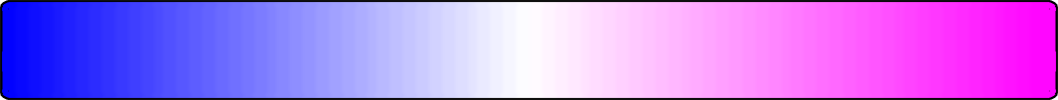
\includegraphics[width=\linewidth,height=0.1in,keepaspectratio]{../bin/colormaps/resource/pymol_blue_white_magenta_spectrum.png}};
        %
        \node(spectrum_bar_loose_label_center)[below, inner sep=5pt] at (spectrum_bar_loose.south) {B-Factor};
        %
        \node(spectrum_bar_loose_label_center)[below, inner sep=5pt] at (spectrum_bar_loose.south east) {200};
        %
        \node(spectrum_bar_loose_label_center)[below, inner sep=5pt] at (spectrum_bar_loose.south west) {1};
    \end{emptypanel}
\end{fullpanelvar}
\caption[Comparing B-factors between tightly-packed and loosely-packed calsequestrin structures]{\textbf{Tightly-Packed Calsequestrin Dimers Consistently Exhibit Increased Conformational Disorder in Domain I, Related to Figure~\ref{fig:intra_dimer_interface}.} The top panel shows tightly-packed calsequestrin dimers (i.e. dimers of calsequestrin crystallized in low pH or with high concentration of multivalent cations). In these structures, solvent-exposed loops in domain I are consistently disordered. In PDB 6OVW, corresponding to this study, the disordered loop region is omitted entirely due to the high level of disorder. This same region (boxed, residues 58-68) is highly disordered in similar structures. The bottom panel shows loosely-packed calsequestrin dimers (i.e. dimers of calsequestrin crystallized at neutral pH with low or trace concentrations of multivalent cations). The resolution for each structure is indicated, and several structures of non-comparable resolution are excluded (2VAF, 5CRE, 5KN0).}
\label{fig:intra_dimer_interface_6OVW_vs_other_B_factor}
\end{figure}
